This chapter describes the goals for the project and the methods employed to achieve them. The first two sections explain the class of similarities between artworks and drawings considered in this project and present examples. Then, the third and fourth section provides a formulation and describes the model architecture along with the data annotation process. The last section details metrics used to evaluate different models.

\section{Problem Statement - Objectives}\label{chap:4:sec:objectives}

Children's drawings contain a rich treasure that gives a peek into their world. Unlike the traditional medical analysis on children's drawings, this project explores them from an Art History point of view by mining the patterns in the drawings that are similar to the historically famous artwork. The digitized collection by the IMAJ - UNESCO center is a miscellany of illustrations from all over the world that vary in drawing techniques and themes. Thus, the problem of matching patterns of renowned works, equally diverse as drawings, in children's drawings translates to a problem of cross-domain image matching or retrieval. 


\begin{figure}
     \centering
     \begin{subfigure}[b]{0.45\textwidth}
         \centering
         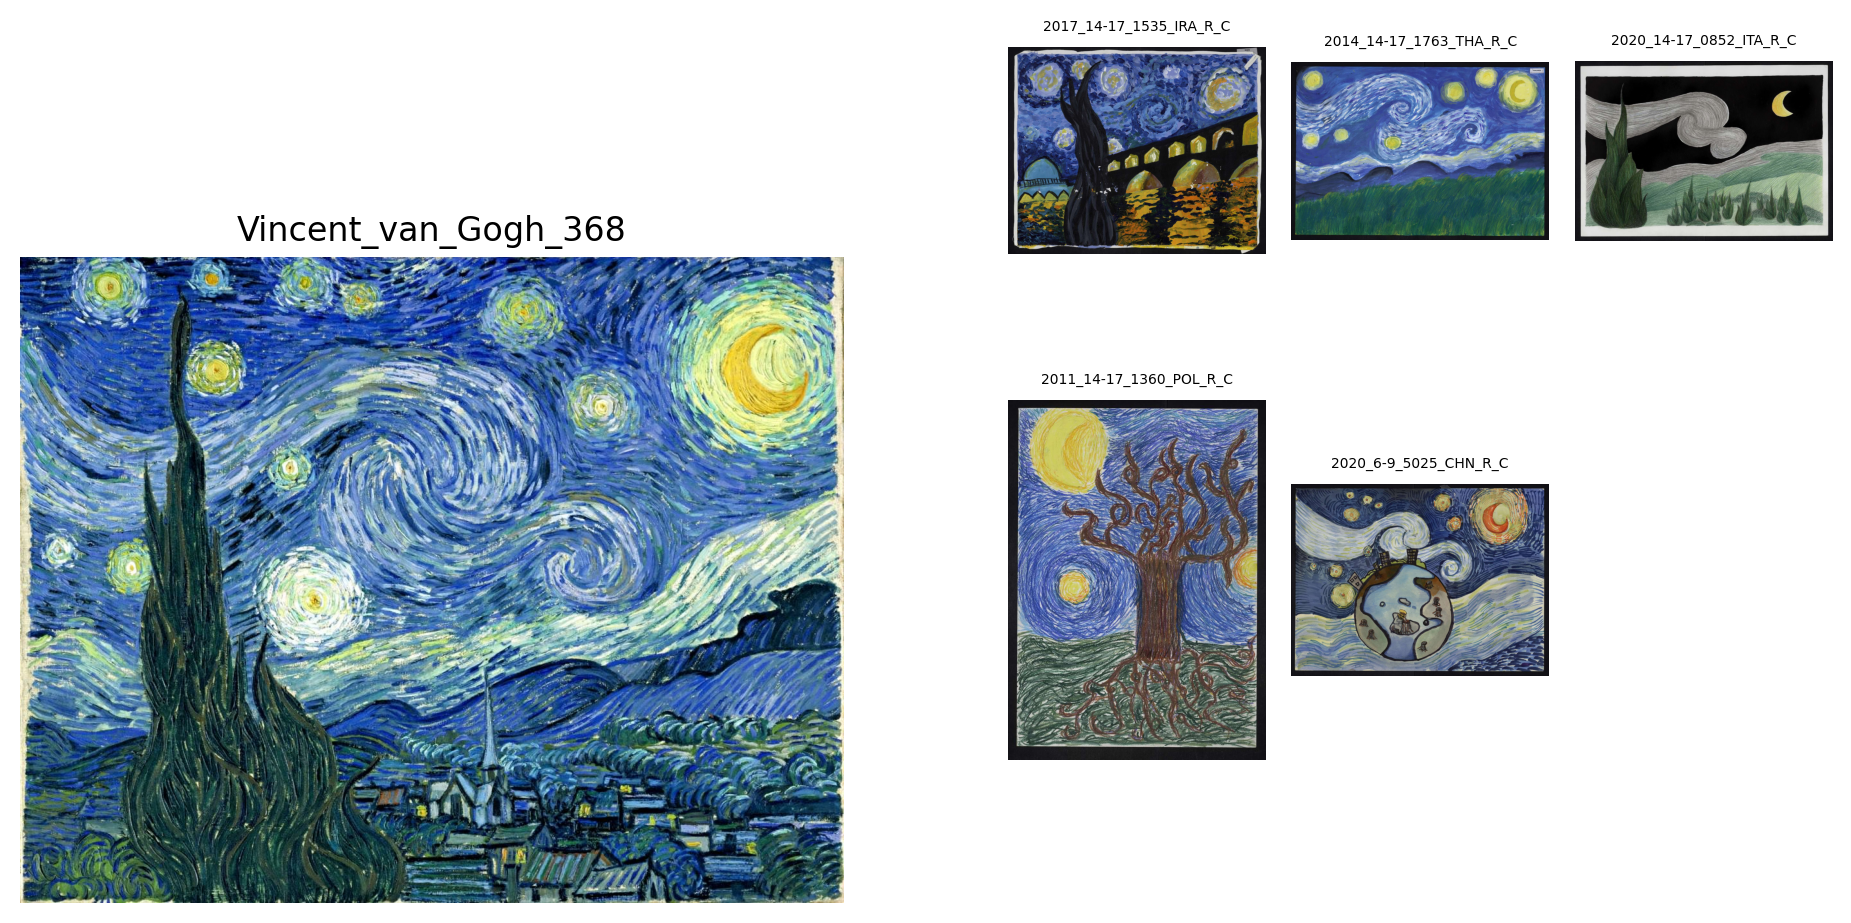
\includegraphics[width=\textwidth]{images/example_pairs/Vincent_van_Gogh_368.png}
         \caption{The Starry Night}
     \end{subfigure}
     \hfil
     \begin{subfigure}[b]{0.45\textwidth}
         \centering
         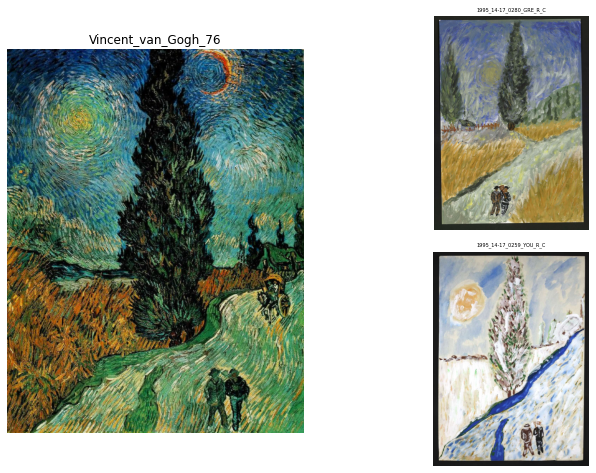
\includegraphics[width=\textwidth]{images/example_pairs/Vincent_van_Gogh_76.png}
         \caption{Road with Cypresses}
     \end{subfigure}
     \hfil
     \begin{subfigure}[b]{0.45\textwidth}
         \centering
         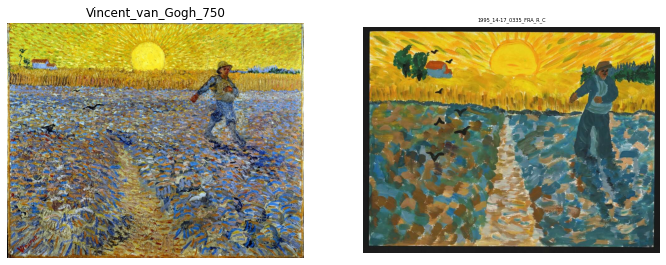
\includegraphics[width=\textwidth]{images/example_pairs/Vincent_van_Gogh_750.png}
         \caption{The Sower}
     \end{subfigure}
     \hfil
     \begin{subfigure}[b]{0.45\textwidth}
         \centering
         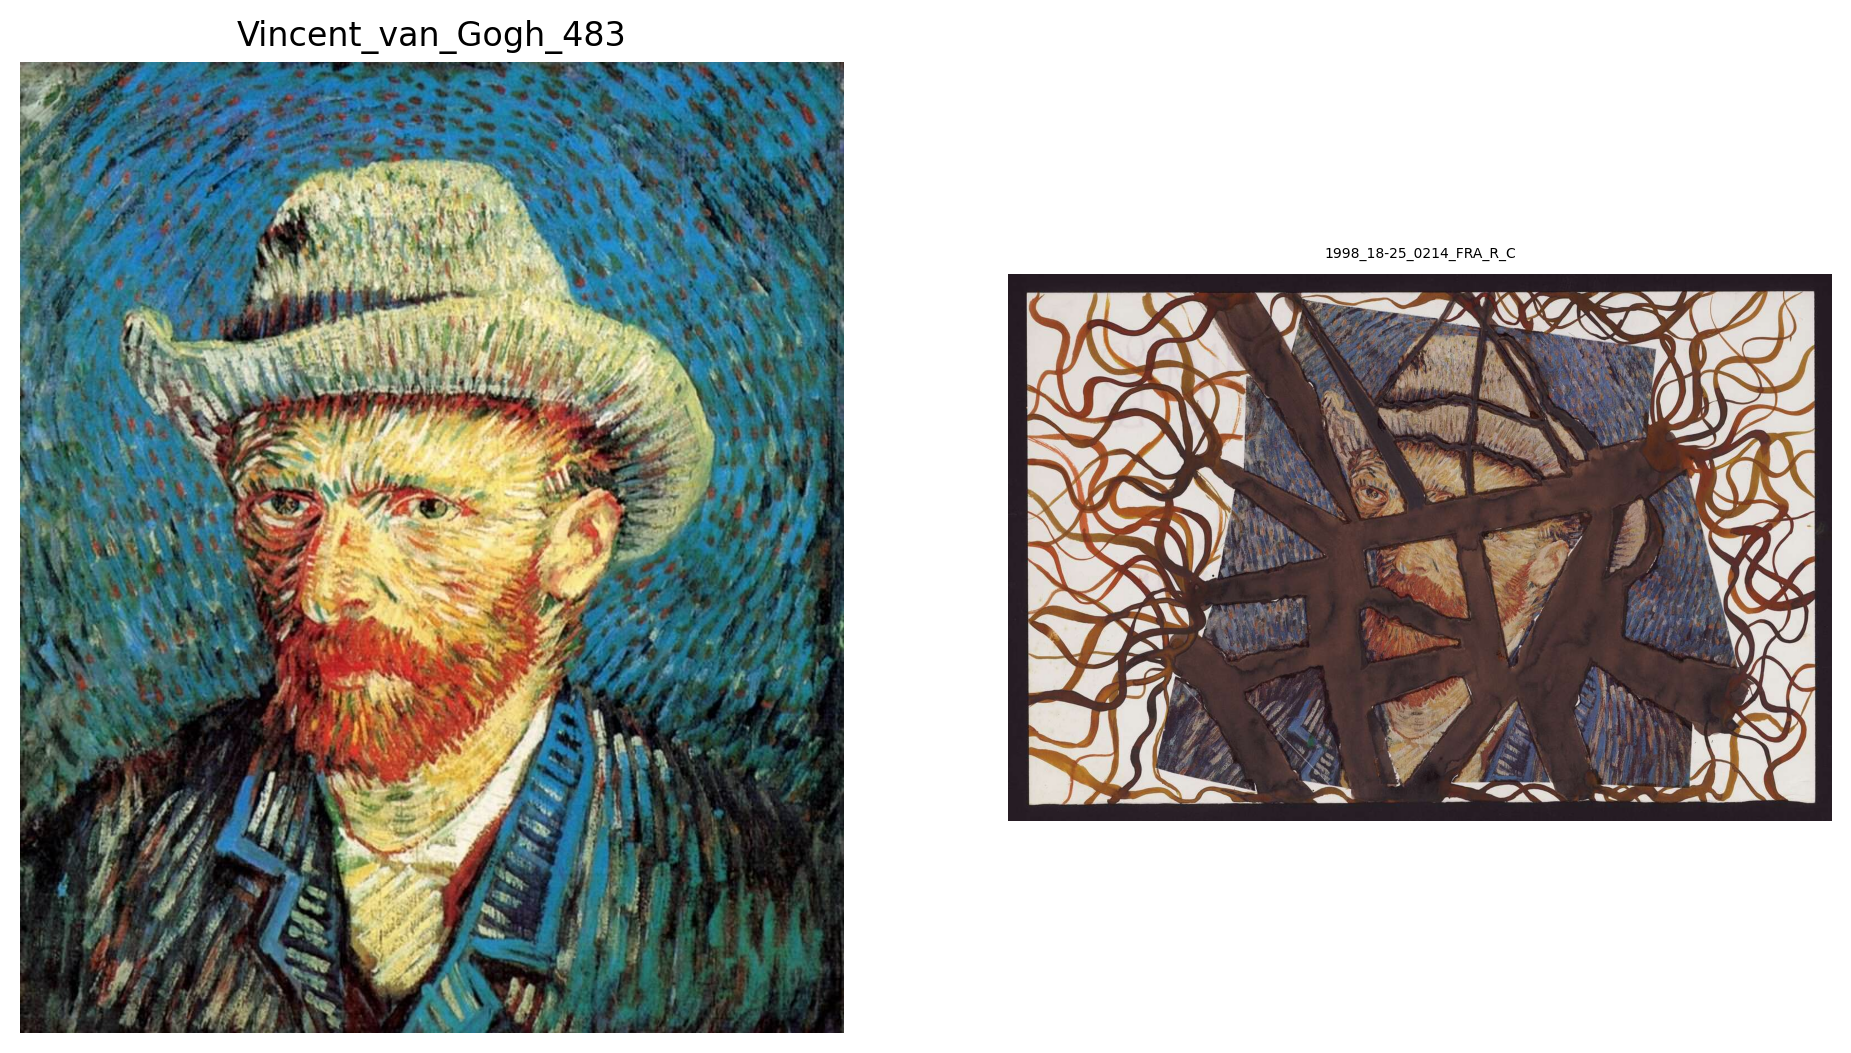
\includegraphics[width=\textwidth]{images/example_pairs/Vincent_van_Gogh_483.png}
         \caption{Self-Portrait with Grey Felt Hat}
     \end{subfigure}
    \caption{Drawings similar to various works of Vincent van Gogh}
    \label{fig:pairs-example-1}
\end{figure}

 \begin{figure}
     \centering
     \begin{subfigure}[b]{0.45\textwidth}
         \centering
         \includegraphics[width=\textwidth]{images/example_pairs/almamy-samory-touré.png}
         \caption{Samori Ture}
     \end{subfigure}
     \hfil
     \begin{subfigure}[b]{0.45\textwidth}
         \centering
         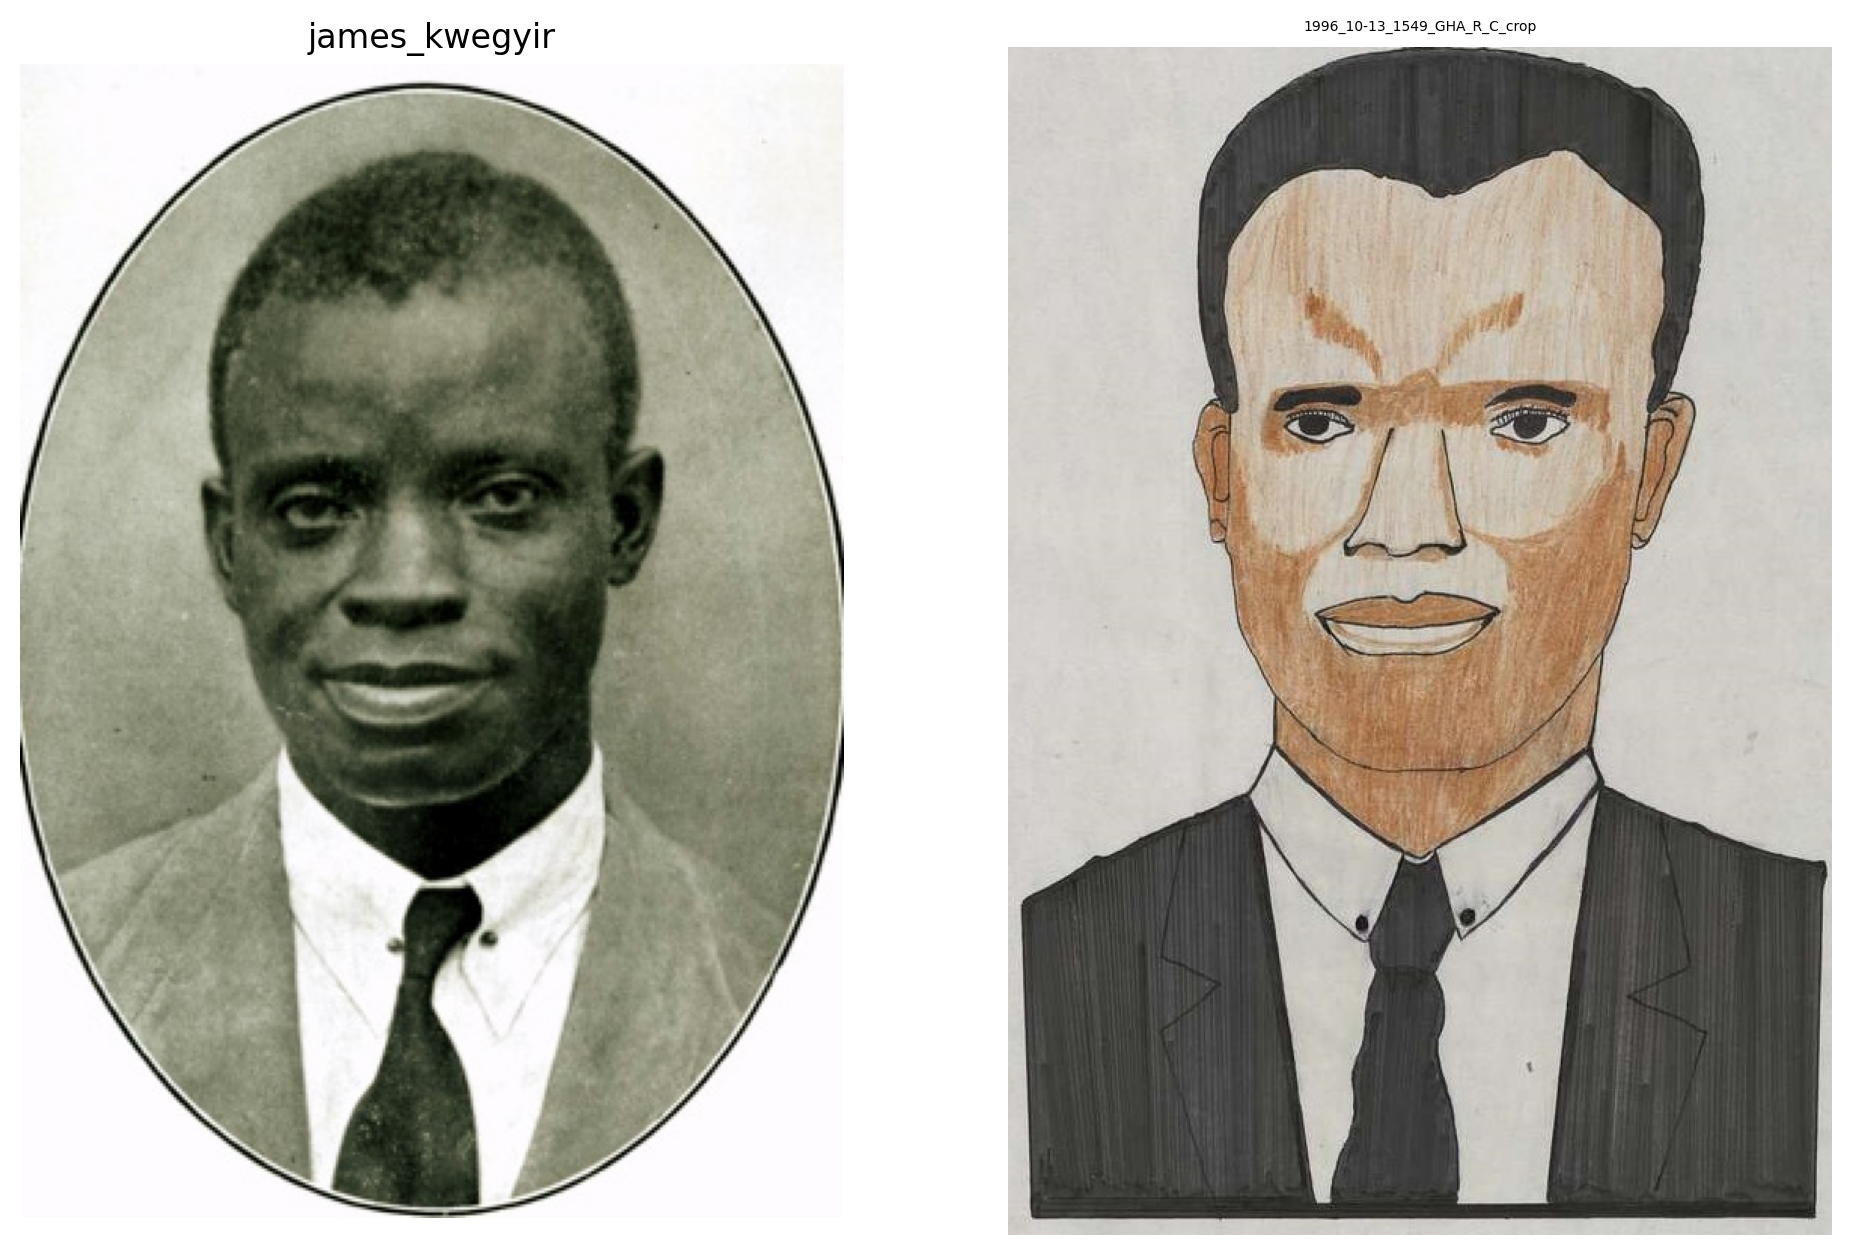
\includegraphics[width=\textwidth]{images/example_pairs/james_kwegyir.png}
         \caption{James Emman Kwegyir Aggrey}
     \end{subfigure}
     \hfil
     \begin{subfigure}[b]{0.45\textwidth}
         \centering
         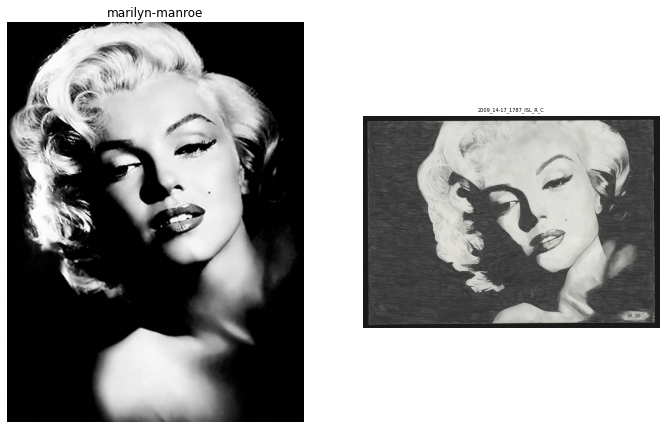
\includegraphics[width=\textwidth]{images/example_pairs/marilyn-manroe.png}
         \caption{Marilyn Monroe}
     \end{subfigure}
     \hfil
     \begin{subfigure}[b]{0.45\textwidth}
         \centering
         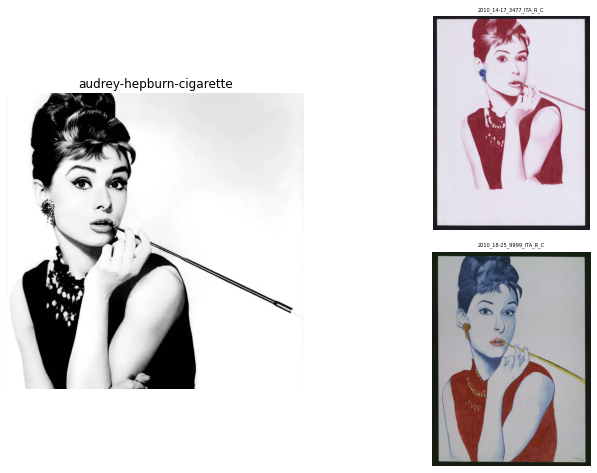
\includegraphics[width=\textwidth]{images/example_pairs/audrey-hepburn-cigarette.png}
         \caption{Audrey Hepburn\footnotemark}
     \end{subfigure}
    \caption{Drawings recreating portraits of famous people}
    \label{fig:pairs-example-2}
\end{figure}

\footnotetext{The first drawing is indeed a copy of the photograph. The drawing competition accepted photos and other digital creations as well.}

\begin{figure}
     \centering
     \begin{subfigure}[b]{0.45\textwidth}
         \centering
         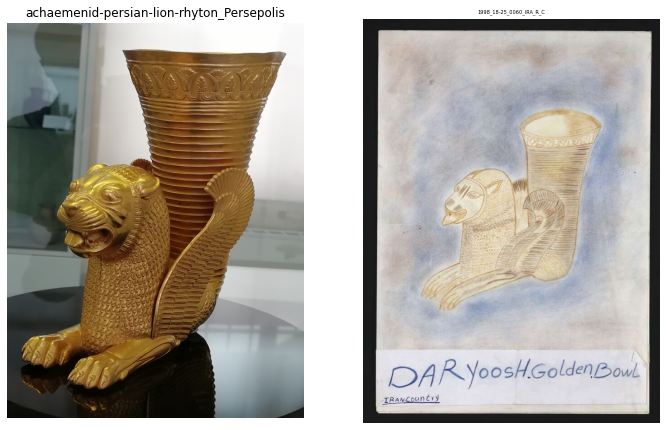
\includegraphics[width=\textwidth]{images/example_pairs/achaemenid-persian-lion-rhyton_Persepolis.png}
         \caption{Achaemenid Persian Lion Rhyton}
     \end{subfigure}
     \hfil
     \begin{subfigure}[b]{0.45\textwidth}
         \centering
         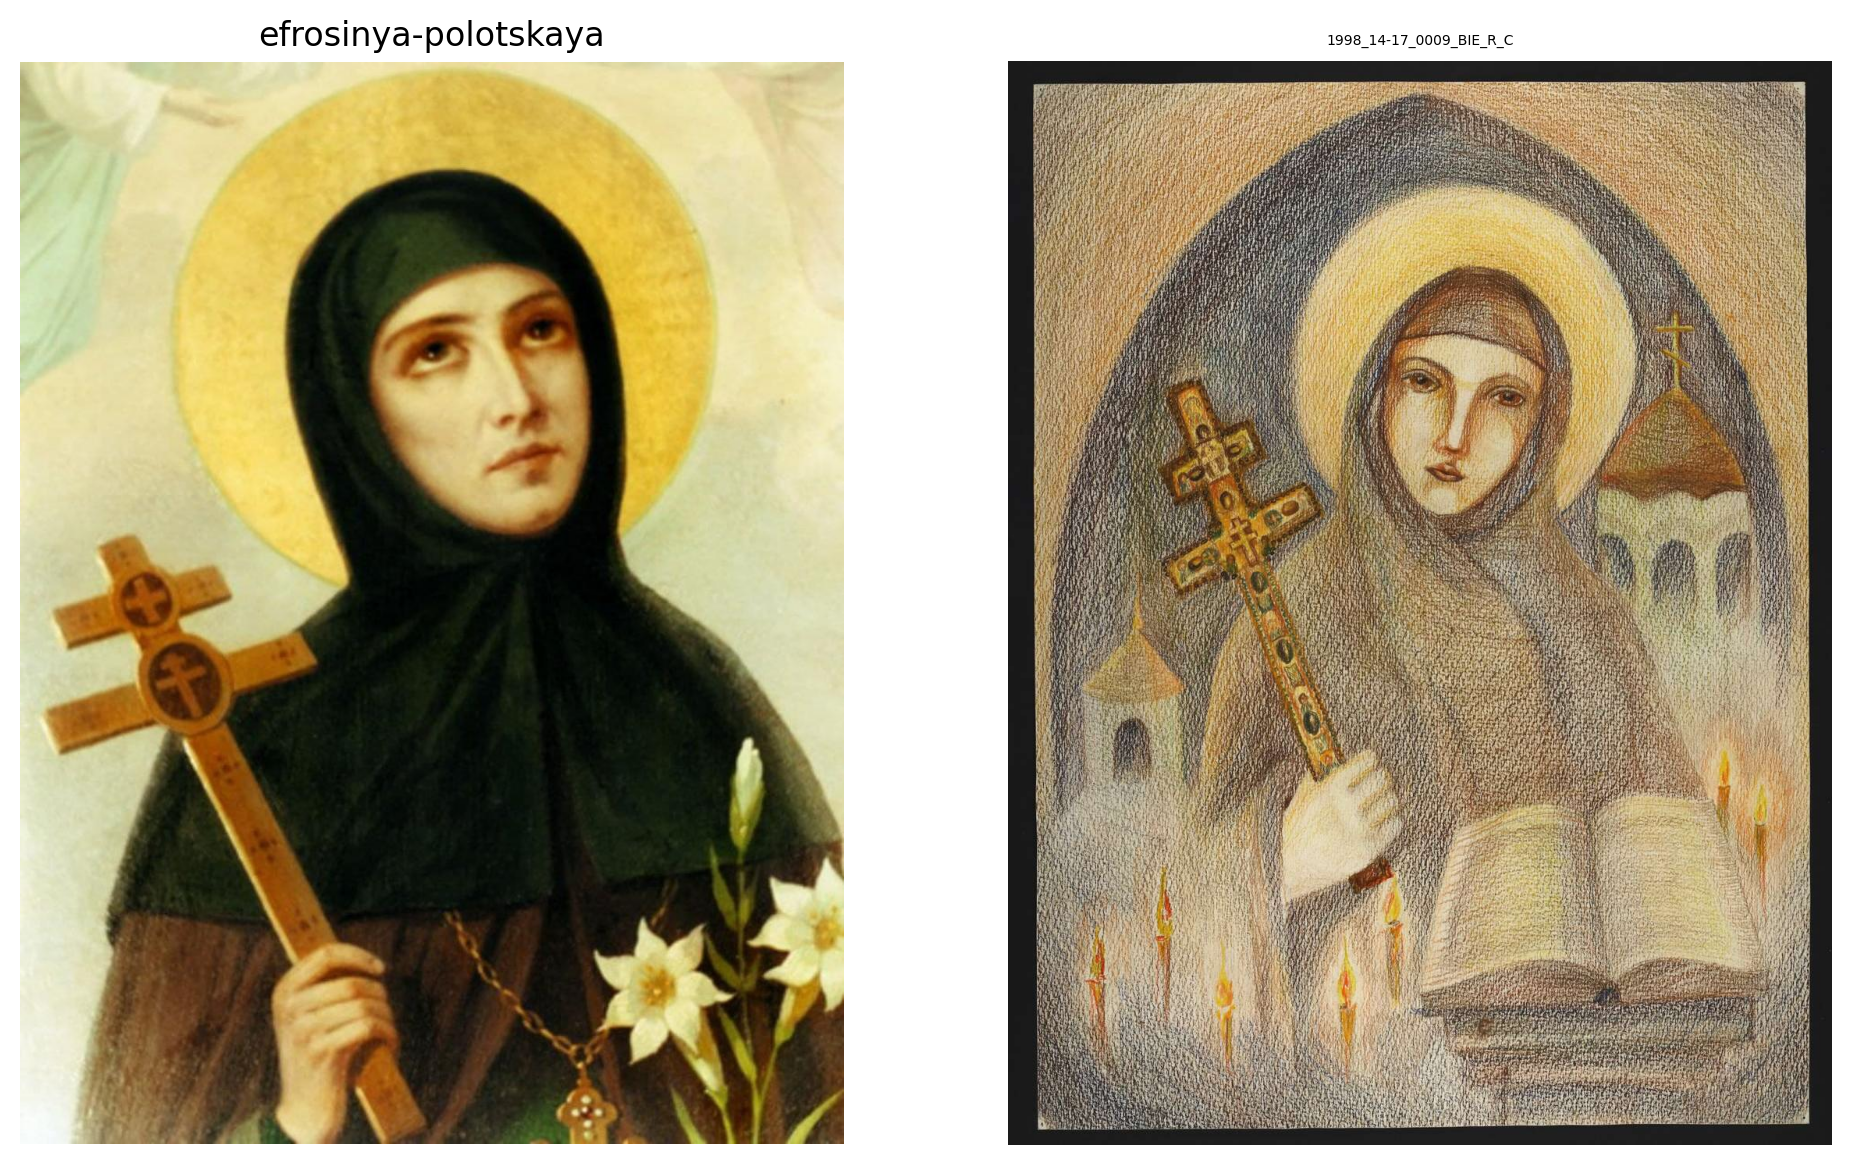
\includegraphics[width=\textwidth]{images/example_pairs/efrosinya-polotskaya.png}
         \caption{Efrosinya Polotskaya}
     \end{subfigure}
     \hfil
     \begin{subfigure}[b]{0.45\textwidth}
         \centering
         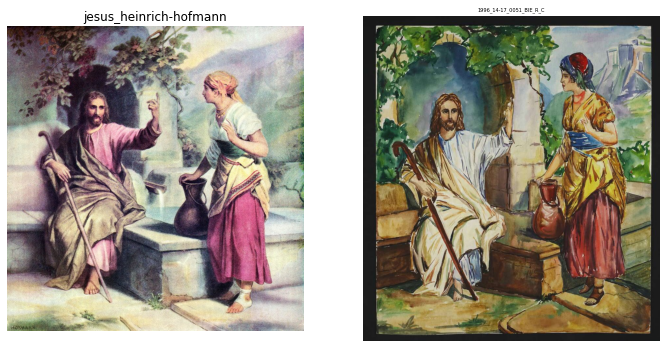
\includegraphics[width=\textwidth]{images/example_pairs/jesus_heinrich-hofmann.png}
         \caption{Jesus and the woman of Samaria}
     \end{subfigure}
     \hfil
     \begin{subfigure}[b]{0.45\textwidth}
         \centering
         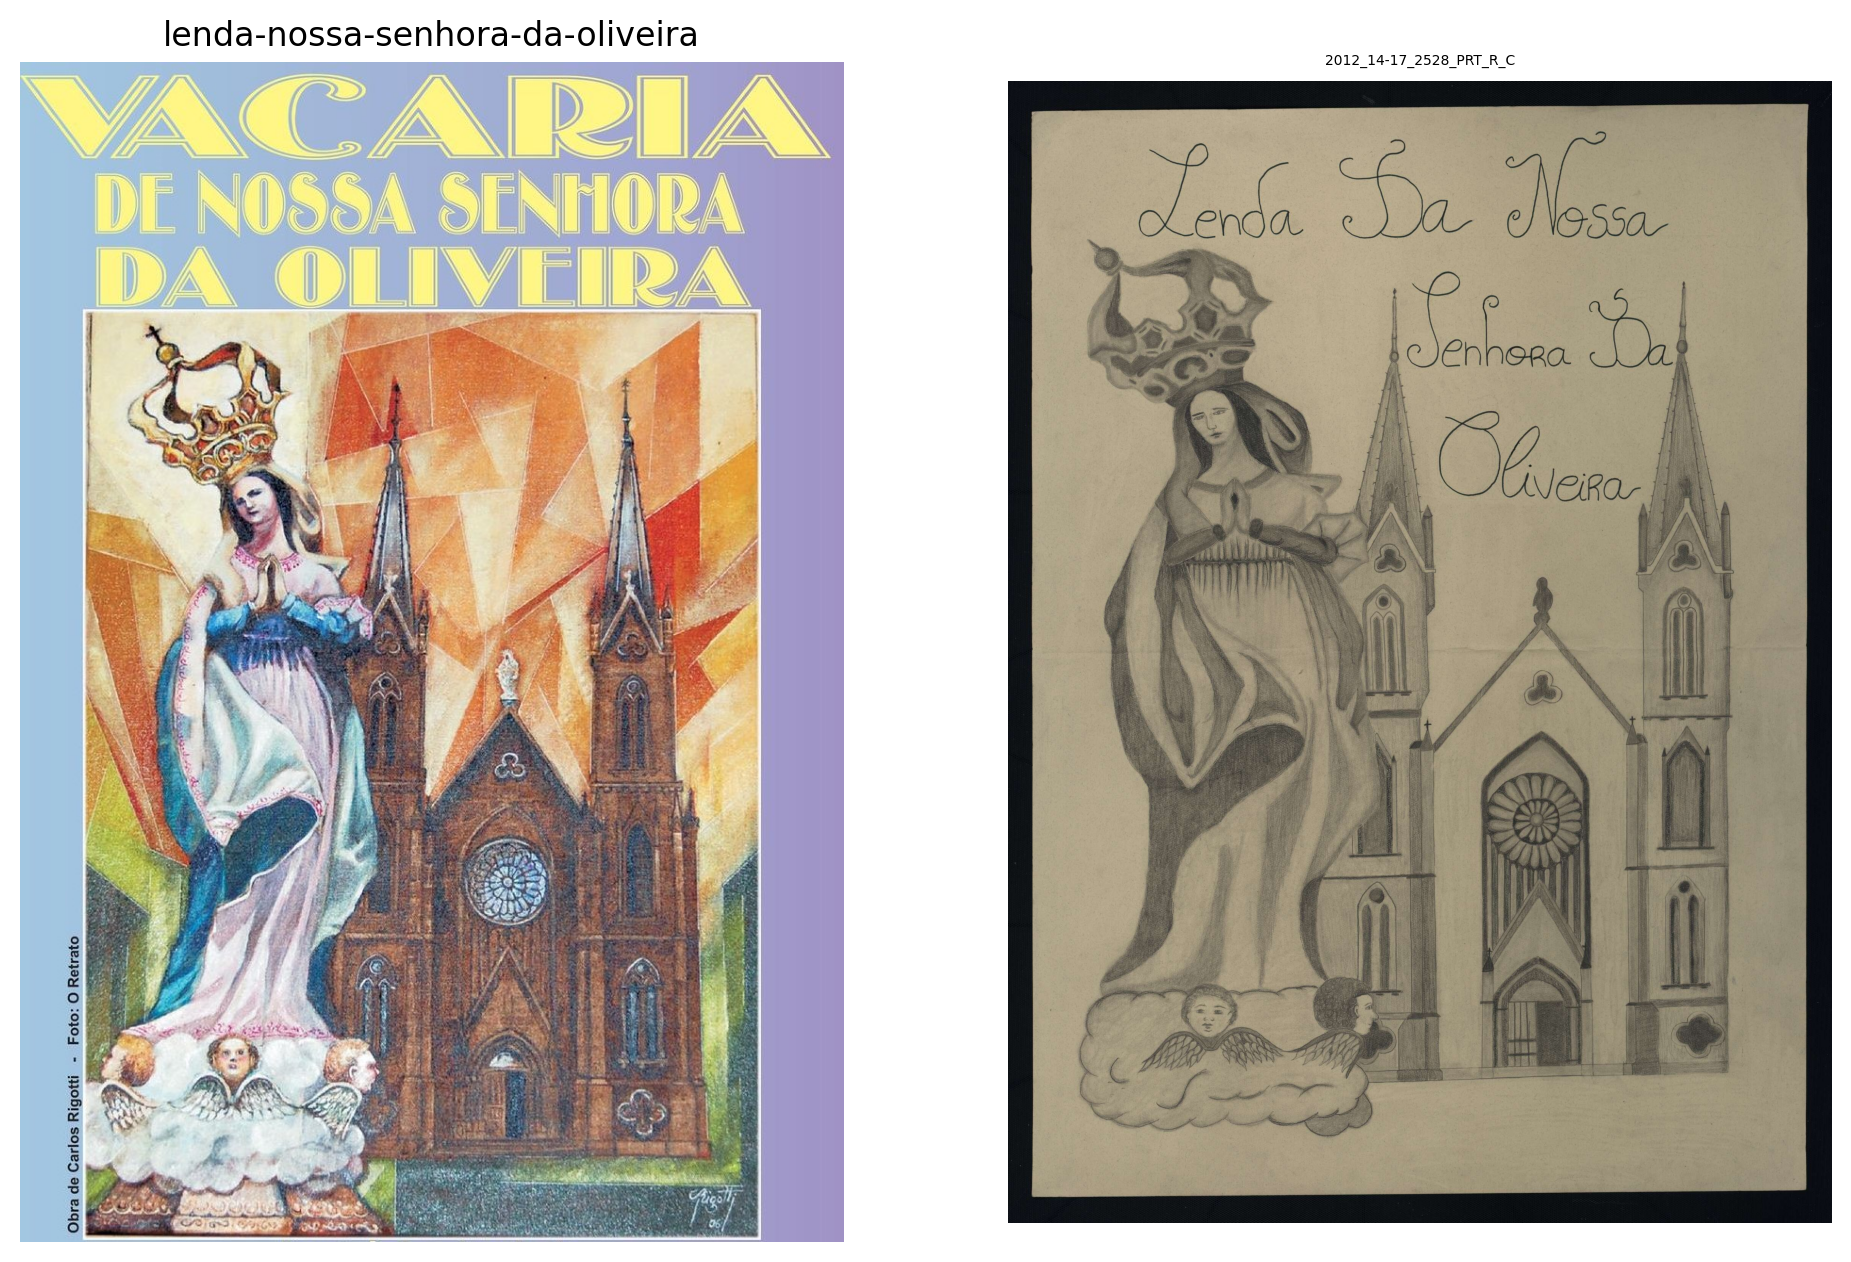
\includegraphics[width=\textwidth]{images/example_pairs/lenda-nossa-senhora-da-oliveira.png}
         \caption{Poster of Nossa Senhora Da Oliveira}
     \end{subfigure}
     \hfil
     \begin{subfigure}[b]{0.45\textwidth}
         \centering
         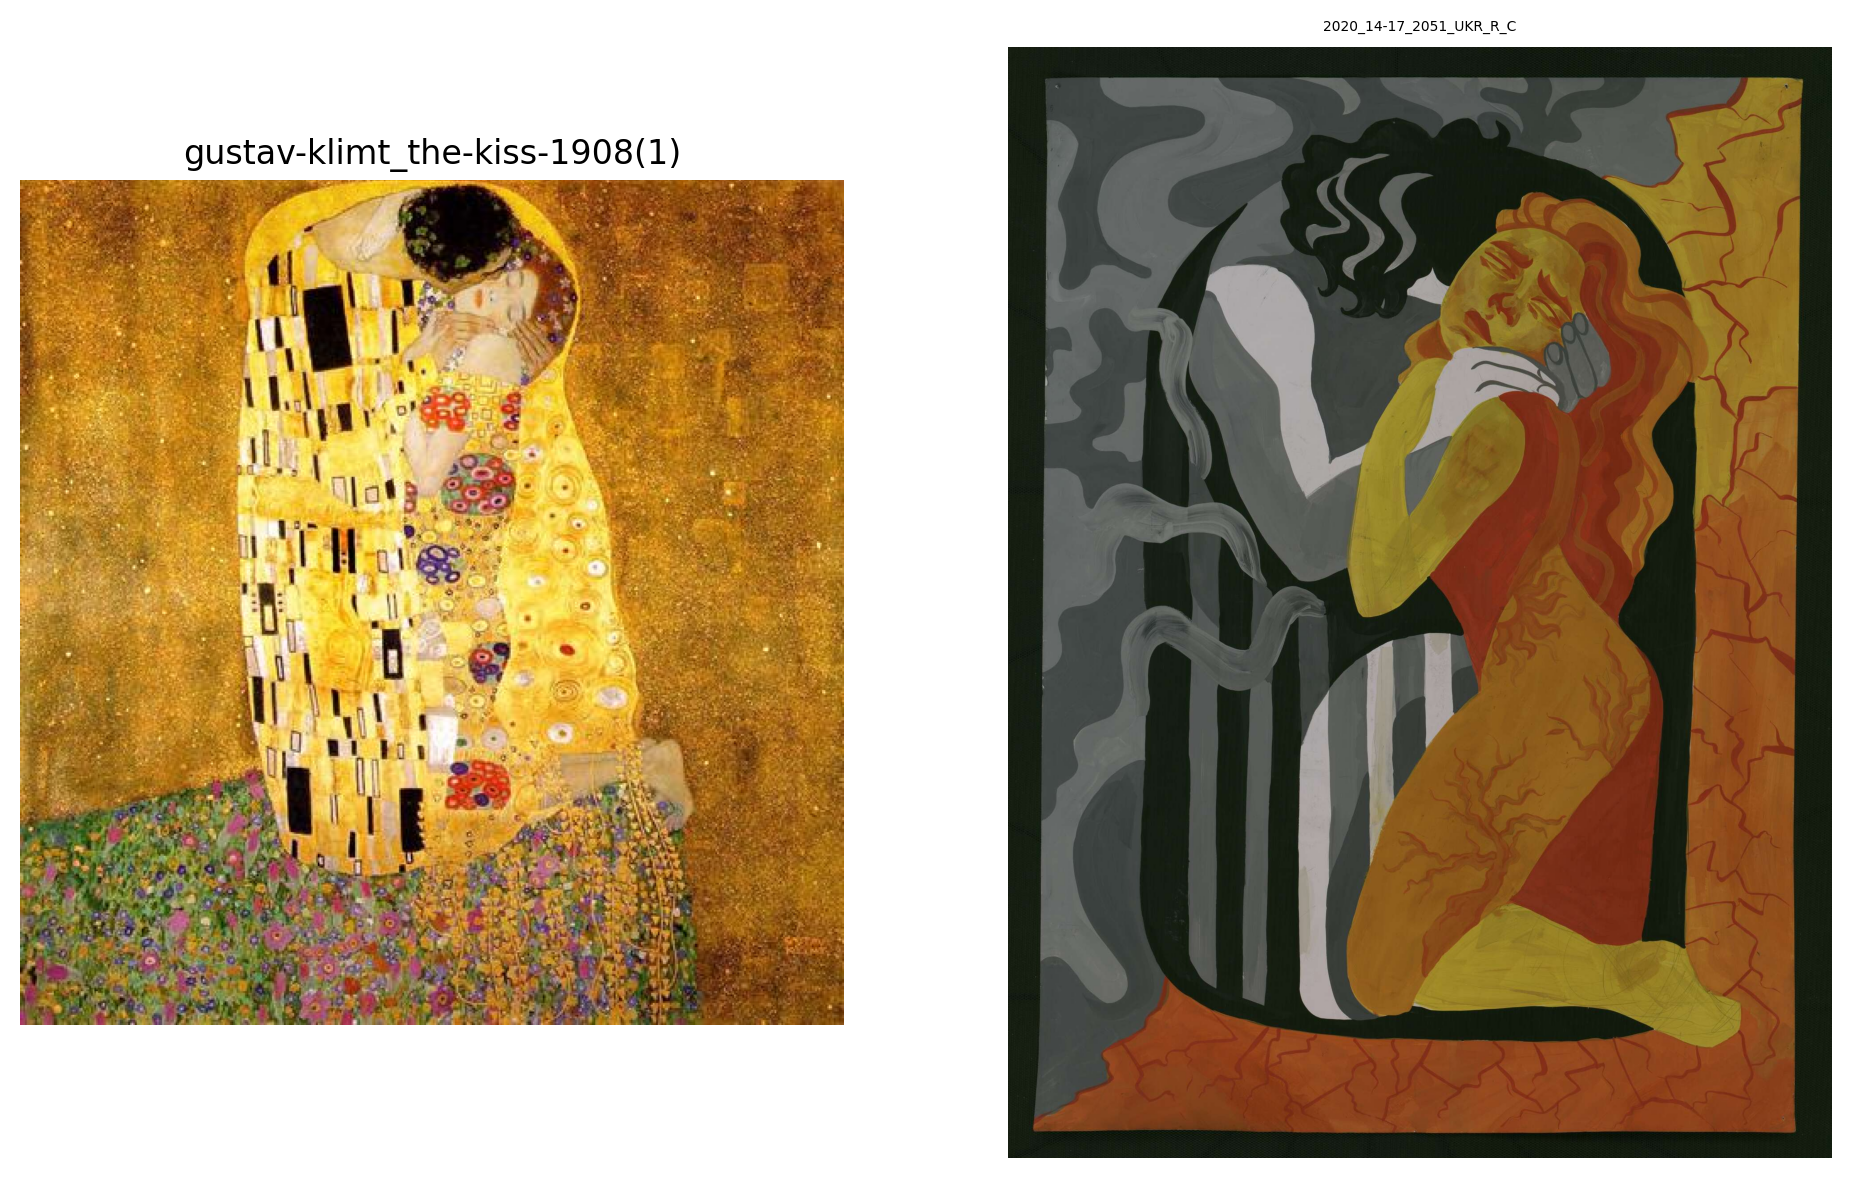
\includegraphics[width=\textwidth]{images/example_pairs/gustav-klimt_the-kiss-1908(1).png}
         \caption{The Kiss by Gustav Klimt}
     \end{subfigure}
     \hfil
     \begin{subfigure}[b]{0.45\textwidth}
         \centering
         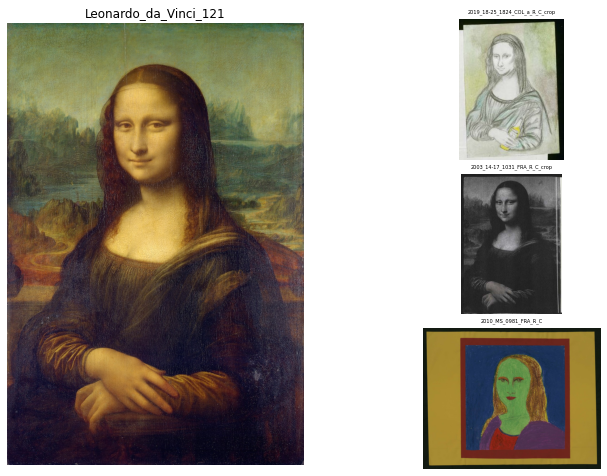
\includegraphics[width=\textwidth]{images/example_pairs/Leonardo_da_Vinci_121.png}
         \caption{Mona Lisa (La Gioconda or La Joconde) by Leonardo da Vinci}
     \end{subfigure}
    \caption{Other sample drawings and the corresponding artworks}
    \label{fig:pairs-example-3}
\end{figure}


Image similarity can mean a spectrum of things ranging from being exact copies to having similar shapes, colors, or subjects of the reference work. Children's drawings and famous artworks are comparable in terms of style, semantic content, nearness of forms, and colors. One can choose and use similarity depending on the research interest, and this work focuses on the re-creation of famous artwork by children. The drawing-artwork pair is said to be similar if the former is a reproduction of the latter, even if the techniques, colors, or domain differ. Figures \ref{fig:pairs-example-1} - \ref{fig:pairs-example-3} shows some example pairs that fall into this category of comparison. The image on the left side of the figure is the artwork similar to the drawing(s) on the right side of the image. Mining these connections can unearth the process of creative creation in children. Namely, it could provide artistic impressions in youngsters and how it varies with age, time, and country.


Additionally, because of the broad-ranging age of children and different levels of expertise and purposes in creating an illustration, the drawings might not replicate the original artwork, requiring to enforce softer thresholds when matching patterns and shapes. All in all, a versatile definition of likeness distinct from the conventional visual searches characterizes similarity in this project, and the corresponding search engine should be invariant to style, medium, color, or shape variations when searching for similar artworks to the children's drawings.

\section{Dataset}\label{chap:4:sec:dataset}

The drawings of children and the popular cultural objects those drawings might have recreated are the two datasets required for this project. While the IMAJ-UNESCO center provided the children's drawings, the cultural objects dataset is primarily composed of the best artworks of 50 influential artists and a few hand-picked examples that were not present in the best artworks dataset.

% \subsection{Children's Drawings}
% Drawings datasets are usually associated with sketch datasets, and commonly used sketch datasets are 
% \begin{enumerate}
% 	\item A crowd-sourced collection of 20,000 sketches belonging to 1000 categories by Eitz et al \cite{eitz2012hdhso}.
% 	\item The Quick-draw dataset contains doodles of 345 objects by players of Google's "Quick, draw" game \cite{jongejan2016quick}.
% 	\item SketchyDatabase with 70,000 pencil sketches paired with the corresponding image \cite{Patsorn2016SketchyDatabase}.
% 	\item A set of 2389 drawings of God(s) by children was presented by Konyushkova et al \cite{Konyushkova2015GodsKD}.
% 	\item Draw-A-Person datasets that collect sketches of a person from children for psychological analysis \cite{Rakhmanov2020ExperimentationOH}.
% \end{enumerate}
% These datasets are useful for tasks of image retrieval, semantic clustering using sketches, generating sketches using deep neural networks or in education, investigating psychology or crime. However, these datasets suffer some drawbacks. First, the top four datasets contain only grayscale pencil sketches, and only the God(s) drawings use colored pencils. Second, the artist's age is available only in the last two datasets. Due to these deficiencies, along with not being child-centric and focusing on a singular object, these datasets are not well suited for the subject of this study which aims to match children's art with cultural objects. The children's drawings from the IMAJ UNESCO center overcome these shortages: they have the artist's age and location information, are not centered on a single object, and are conceived using different methods and materials. Chapter 3 discusses the dataset in detail. 
 

\subsection{Famous Artworks Dataset}

A dataset of reference cultural entities is equally essential as the dataset of children's drawings for this project. As mentioned in Section \ref{chap:1:sec:children-art-analysis}, these cultural objects include multiple kinds of visual arts. Nevertheless, due to the nature of the competition and the type of institutes that participate in the competition, historically famous paintings constitute the primary component of the reference set. Table \ref{table:artworks-datasets} lists a few online paintings archives (presented in \cite{seguin_2016}) suitable for this project.

\begin{table}[ht]
    \centering
    \begin{tabular}{|p{0.2\linewidth}|p{0.7\linewidth}|}
    \hline
        \textbf{Dataset} & \textbf{Mini-Description} \\ \hline
        \textbf{Web Gallery Of Art} \cite{wga} & Database of more than 52,000 European fine arts from the Baroque, Gothic, and Renaissance periods. \\ \hline
        \textbf{Wikiart} \cite{wikiart} & Online visual arts database that contains around 250,000 artworks from museums, universities, and civic buildings. \\ \hline
        \textbf{Rijksdata} \cite{mensink14rijkschallenge} & Dataset of nearly 112,000 photographs of artworks at the Rijksmuseum. Mensik and Germet presented the dataset and baseline scores for predicting the creator, material, type, and year of artworks.\\ \hline
        \textbf{Best Artworks Of All Time} \cite{icaro19baat} & Hand-curated dataset of 8355 works of the most influential artists. The dataset was scraped from the Art Challenge website \cite{ruben_anna_2014} and published on Kaggle by a user. \\ \hline
    \end{tabular}
    \caption{Descriptions of datasets of reference artworks}
    \label{table:artworks-datasets}
\end{table}

Each dataset in Table \ref{table:artworks-datasets} contains a great set of works in terms of quantity and variety, but the current project uses the Best Artworks of All Time (BAAT) dataset to compare the children's drawings. The reasons for choosing the BAAT dataset are 
\begin{enumerate}
	\item it contains the paintings of influential artists, increasing the probability of recreating their works, and
	\item using a smaller dataset makes the solution computationally faster. Nevertheless, the solution is independent of the reference dataset.
\end{enumerate}

BAAT dataset contains photographs of 8446 artworks created by the 50 most influential artists\footnote{The choice of influential artists is not universal and could differ among individuals. This thesis considers the dataset as it is without delving into the debate of the correctness of the artists' selection.} from 18 nations. The genres of the works include Renaissance, Byzantine Baroque, Realism, Impressionism, Pop Art, Primitivism, Surrealism, Social Realism, Muralism, Expressionism, Cubism, and Neoplasticism. After going through the children's drawings, 131 photos of people, places, animals, and paintings that were not present before supplemented the BAAT dataset, increasing the total count to 8557. Section \ref{chap:4:data-anno} describes the steps in obtaining these additional images, and they are similar to a few drawings in the dataset.

\section{Approach}\label{chap:4:sec:algo}

The basic idea to solve the problem of pattern matching in children's drawings (hereon drawings) and famous artworks (hereon artworks) was to use the distances between their feature vectors and perform a nearest neighbor search. A deep neural network system using a CNN to extract features of the images and a metric learning strategy to train the network implements the core solution. The decision to use a CNN stems from the previous results on their capabilities in image retrieval tasks \cite{wan2014deep} and particularly from the findings of \cite{seguin_2016}, where the authors reported that CNNs perform significantly better than the classical Bag-of-Words methods that use local descriptors like SIFT for a similar type of task.

Popular CNNs architectures trained for image classification tasks are publicly available as pre-trained models/networks. Although pre-trained models learn general features in images, their performance in image retrieval tasks compared to object classification is minimal. The retrieval capability further worsens in the cross-domain search of drawings and artworks, providing scope for improvement. However, the lack of a large labeled dataset of drawing and artwork pairs, such as ImageNet for classification, makes it hard to train a deep learning model for the specific task. At the same time, the standard distance measures do not capture the class of similarity this project aims to find between the images, and it is also challenging to design a suitable metric for such a task. Metric learning helps construct this distance metric, and training a CNN model using that metric optimizes the image embeddings enabling a comparison between them. Therefore, using the Transfer learning process, a pre-trained model is fine-tuned by employing a triplet learning approach.

\subsection{Feature Extraction}

ResNeXt CNN architecture \cite{Xie2016} acts as the base network for feature extraction in this project. In particular, the ResNeXt-101 architecture, where 101 implies the number of layers, is used. The selection of ResNeXt-101 results from the analysis in \cite{Seguin2018MakingLA}, that suggests newer architectures and high-dimensional feature vectors provide better performance compared to low-dimensional feature vectors. ResNeXt is a relatively modern architecture that combines the features of ResNet and Inception Net and produces a feature vector of size 2048. The intuition of using a high-dimensional feature vector is that it could hold more information about the image. 

Although it is possible to create a new CNN architecture, reusing already proven existing architectures is preferred, and it gives a possibility for Transfer Learning. For each image, a fixed-length vector of dimension 2048 is obtained by average pooling the activation output of the last convolutional layer in ResNeXt-101. The fixed-length vector is then \begin{math} l^2 \end{math}-normalized to create a feature vector.

\subsection{Quantification of Similarity}

While CNNs can produce image feature vectors, a distance function is needed to compare them. This distance (or similarity) function should accept the feature vectors as input and output the distance (or similarity) between them. A commonly used metric to compare high dimensional vectors is Cosine Similarity, as it is simple and independent of the magnitude of the values in the vector.

Cosine Similarity is the cosine of the angle between the vectors and lies in the range \begin{math} [-1,+1] \end{math}. With this definition, the similarity is \begin{math} +1 \end{math} for proportional vectors as the angle between them is zero, \begin{math} -1 \end{math} for vectors that are \begin{math} 180^\circ \end{math} (degrees) apart, and \begin{math} 0 \end{math} for orthogonal vectors - perpendicular to each other. If two vectors are similar, their cosine similarity is \begin{math} 1 \end{math}, and the distance should be \begin{math} 0 \end{math}. Thus, the cosine distance is defined as \begin{math} 1 - Cosine \ Similarity \end{math}. This work uses the cosine distance to estimate the nearness between the images, i.e., the \textit{distance function} (See Section \ref{chap:2:metric-learn})
\begin{equation*}
\begin{split}
dist(\pmb{x}, \pmb{y}) = 1 - cos(\pmb{x}, \pmb{y}) \\
= 1 - \frac {\pmb{x} \cdot \pmb{y}}{||\pmb{x}|| \cdot ||\pmb{y}||} \\
= 1 - {\pmb{x} \cdot \pmb{y}}
\end{split}
\end{equation*}
where \begin{math} \pmb{x}, \pmb{y} \end{math} are the \begin{math} l^2 \end{math}-normalized feature vectors of two images.
Therefore, the artworks similar to the drawings should have lower distances than the unrelated artworks.


\subsection{Data Annotation}\label{chap:4:data-anno}

A crucial step in the training process is to map the drawings and similar artworks to create an anchor and positive pairs to use in triplet learning. All the children's creations do not necessarily recreate a well-known art. Moreover, there is no pre-existing mapping between the IMAJ UNESCO center drawings and BAAT dataset, or for that matter, any reference dataset, resulting in the manual annotation of drawings and artworks pairs. After a visual inspection, the current project uses the works of only the 14-17 and 18-25 age groups, as the drawings in the very young ages are scribbles and other age categories have few references to famous artworks. There are 19,777 drawings in the combined 14-25 age group, and they were surveyed to identify a reference artwork using a three-step process.

The first step deals with the clear cases by either pairing them with familiar artworks or discarding them if there is no apparent reference. The majority of the drawings fall into the latter category. In the second step, a few ambiguous drawings are searched online using the reverse image search on Google Images\footnote{https://images.google.com/}. The reverse image search revealed very few references. Lastly, a text-based search using the title or description or the location of the artist available on the verso side of the non-obvious drawings helped uncover a couple of references/inspirations. Examining 8800 drawings (44\%) in steps 2 and 3 resulted in identifying 208 possible references between 194 (2.2\% of 8800) drawings and 151 artworks. Out of the 208 possible pairs, 77 were not forthright and overreaching in some cases. Scrapping the 77 ambiguous pairs leaves with 131 anchor and positive duos between 127 drawings and 100 artworks.


\subsection{Algorithm}

\begin{figure}[ht]
\centering
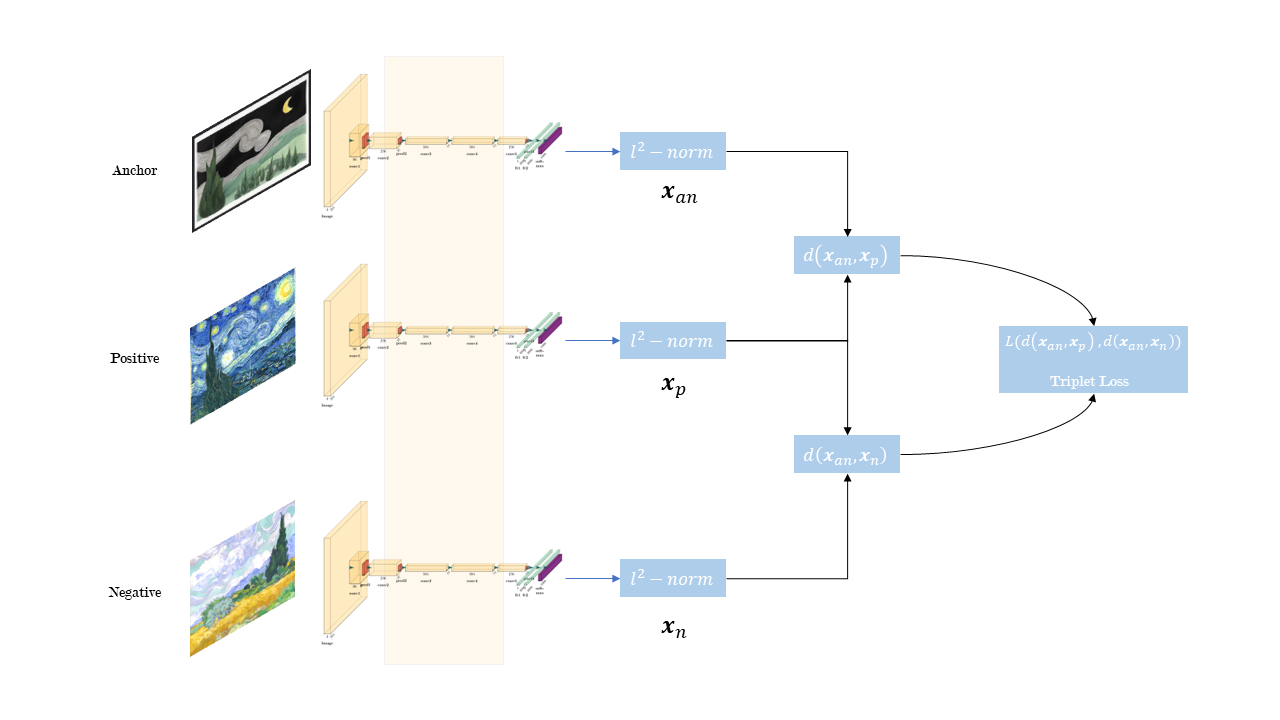
\includegraphics[width=\textwidth]{images/triplet_network/triplet_learning.png}
  \caption{Schema for the model training using triplets. Adapted from \cite{Seguin2018MakingLA}. The same network process all the images; thus, all the networks share the same parameters. Each image is processed, converted into a 2048 dimension vector, and normalized. The network parameters are updated using the triplet loss (\begin{math} L \end{math}), where \begin{math} d \end{math} is the distance function.}
  \label{fig:triplet-network}
\end{figure}


Figure \ref{fig:triplet-network} lays out the model schema where CNN processes the images and is optimized based on the difference in distance between the images. The triplet learning method requires three inputs (Anchor (an), Positive (p), and Negative (n)), three images in this case. The anchor image is a child's drawing, and the positive and negative images are artworks similar and dissimilar to the anchor, respectively. The dependency between the mining of triplets and the distance function makes the model training an iterative process. Its summary is in Pseudocode \ref{alg:modeltrain}.


\begin{algorithm}
\caption{Pseudo algorithm for the model training}\label{alg:modeltrain}
\begin{algorithmic}[1]
\State Initialize a pre-trained CNN (ResNeXt) truncating the fully connected layers at the end to produce a feature vector to the input. \\ The CNN network symbolizes the distance function \begin{math} dist \end{math}.
\While {\begin{math} dist(\pmb{x}_{an}, \pmb{x}_{n}) + \tau < dist(\pmb{x}_{an}, \pmb{x}_{p}) \end{math} for any \begin{math} (an, p) \end{math} pair}
	\State For each \begin{math} an \end{math} and \begin{math} p \end{math}, mine for \begin{math} N_{T} \end{math} number of \begin{math} n \end{math}'s using the feature vectors obtained from the CNN network to create a Triplets set
        
    \begin{math}
    T = \{(an, p, n) : an \in D, p \in A, and \{n \in A: \lvert \{ n^{\prime} \in A : dist(\pmb{x}_{an}, \pmb{x}_{n}) < dist(\pmb{x}_{an}, \pmb{x}_{n^{\prime}})) \} \rvert < N_{T} \} \}
    \end{math}
	\State Calculate the Triplet loss for \begin{math} T \end{math} using Equation \eqref{triplet_loss}
		\State Compute an average of the loss over all \begin{math} (an, p) \end{math} pairs.
	\State Backpropagate and update the CNN network using the triplet loss
\EndWhile
\end{algorithmic}
\end{algorithm} 

\section{Usage}\label{chap:4:sec:usage}

Deploying the model to explore the connections between a fixed set of drawings and artworks is simple and available offline as all the feature vectors can be computed once and stored. However, an iterative loop of adding new connections, fine-tuning the model, and exploring and identifying further similar pairs is possible. First, the trained CNN is used to compute the feature vectors for all images in both datasets. Arranging the artworks in the ascending order of their cosine distance from the drawing produces a ranking of similarities, and the top ones should be the relevant artwork for the drawing.

\section{Evaluation Metrics}\label{chap:4:sec:metrics-descrp}

The metrics used to compare and evaluate the model's performances fall into two categories. The position of the relevant artwork for a drawing in the retrieved list will assist in tracking the learning of the models. On the other hand, the recall and precision values at different positions assess the performance of the models. Due to the limited availability of data, there is a possibility of obtaining a result that fits specific drawing-artwork pairs. Thus, it is necessary to estimate the uncertainty of the model and the quality of the results. This work uses a 11-Fold Cross-Validation to assess a model, where eleven different train, validation, and test data splits evaluate the model. The reported metrics result from averaging the results of all eleven splits.

\subsection{Mean Position}

The aim of training a retrieval model is that when queried with a drawing, the relevant artwork(s) should have the least distance and appear in the first place(s). Monitoring the change in the retrieved position of artwork enables seeing how early the relevant artworks appear in the retrieval list and how it changes as the model is updated. An average of such rank for all drawings in a set gives a single metric to track the change. A low average position implies that the model rates the similar artworks closer to the query than the dissimilar ones. 

If \begin{math} a \end{math} is an artwork in the set of artworks (\begin{math} A \end{math}), \begin{math} d \end{math} is a drawing in the set of drawings \begin{math} D \end{math}, and \begin{math} {A}_{d} \end{math} is the set of relevant artworks for drawing d. The average position of a set of drawings (\begin{math} MP \end{math}) is defined as
\begin{displaymath} 
MP = \frac{1}{\left | D \right |}\sum_{d\varepsilon D, {d}_{a} \varepsilon {A}_{d}} (Rank({d}_{a}, {A}_{Md}))
\end{displaymath}
where \begin{math} {A}_{Md} \end{math} is the list of artworks (\begin{math} A \end{math}) ordered in increasing order of distance with respect to \begin{math} d \end{math} and \begin{math} Rank \end{math} is function that accepts the ordered artworks and the relevant artwork to output the position of \begin{math} {d}_{a} \end{math} in \begin{math} {A}_{Md} \end{math} in the range of \begin{math} [0, \left | A \right | - 1 ] \end{math}.

\subsection{Recall}\label{chap:4:sec:metrics-descrp:recall}

Recall facilitates assessing the relevance of the results to the query. It provides the percentage of relevant artworks in the retrieved list. However, since the model ranks all the artworks based on the distance, the recall reaches \begin{math} 100\% \end{math}. Hence, recall at different ranks is computed by limiting the number of results taken into account to calculate it. Recall@k is the share of relevant artworks in the top-k-ranked artworks.

The recall up to a rank \begin{math} k \end{math} for a set of drawings (\begin{math} {Recall@k} \end{math}) is the average recall up to a rank \begin{math} k \end{math} for each drawing in the set 
\begin{displaymath}
{Recall@k} = \frac{1}{\left | D \right |}\sum_{d\varepsilon D}Recall@k(d)
\end{displaymath}
and 
\begin{displaymath}
Recall@k(d) = \frac{ \left | \{ \{ A_{Mdi} | i \leq k \} \cap {A}_{d} \} \right |} { \left | {A}_{d} \right |}
\end{displaymath}

\subsection{Mean Average Precision}

While recall gives the share of relevant artworks in the retrieved, precision provides the percentage of relevant retrieved artworks. As all the artworks are ranked using the cosine distance to the drawing, similar to the \begin{math} Recall@k \end{math}, \begin{math} Precision@k \end{math} is more relevant, and the Average Precision (AP) aggregates the precisions at all positions. 

The Mean Average Precision (MAP) for a set of drawings is the average of the average precision for each drawing in the set,
\begin{displaymath}
MAP = \frac{1}{\left | D \right |}\sum_{d\varepsilon D} {AP}_{d}
\end{displaymath}

\begin{displaymath}
{AP}_{d} = \sum_{k=1}^{\left | {A}_{d} \right |} Precision@k(d) * (Recall@k(d) - Recall@k-1(d))
\end{displaymath}

\begin{displaymath}
Precision@k(d) = \frac{ \left | \{ \{ A_{Mdi} | i \leq k \} \cap {A}_{d} \} \right |} { \left | \{ A_{Mdi} | i \leq k \} \right |}
\end{displaymath}